\documentclass[10pt]{article}
\usepackage{tikz}
\usetikzlibrary{shapes.misc}
\usepackage[margin=0cm]{geometry}
\pagestyle{empty}
\tikzstyle{every node}=[cross out, draw, red]

\begin{document}

\vspace*{\fill}
\begin{center}
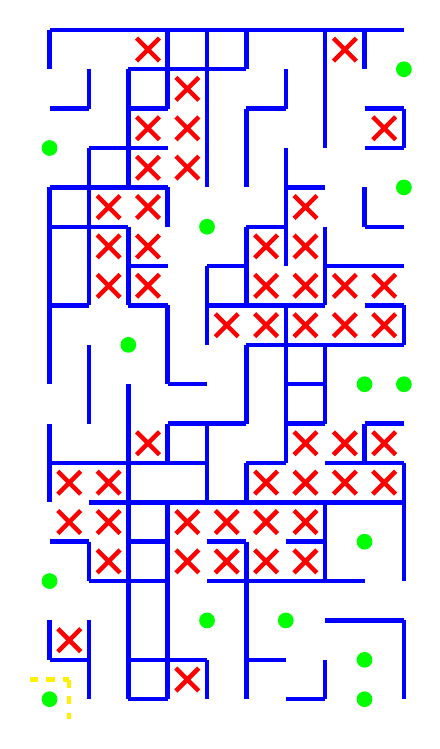
\begin{tikzpicture}[x=0.5cm, y=-0.5cm, ultra thick, blue]
% Walls
    \draw (0,0) -- (9,0);
    \draw (2,1) -- (5,1);
    \draw (0,2) -- (1,2);
    \draw (2,2) -- (3,2);
    \draw (5,2) -- (6,2);
    \draw (8,2) -- (9,2);
    \draw (1,3) -- (3,3);
    \draw (8,3) -- (9,3);
    \draw (0,4) -- (3,4);
    \draw (6,4) -- (7,4);
    \draw (0,5) -- (2,5);
    \draw (5,5) -- (6,5);
    \draw (8,5) -- (9,5);
    \draw (2,6) -- (3,6);
    \draw (4,6) -- (5,6);
    \draw (7,6) -- (9,6);
    \draw (0,7) -- (1,7);
    \draw (2,7) -- (3,7);
    \draw (4,7) -- (7,7);
    \draw (8,7) -- (9,7);
    \draw (5,8) -- (9,8);
    \draw (3,9) -- (4,9);
    \draw (6,9) -- (7,9);
    \draw (3,10) -- (5,10);
    \draw (6,10) -- (7,10);
    \draw (8,10) -- (9,10);
    \draw (0,11) -- (4,11);
    \draw (5,11) -- (6,11);
    \draw (7,11) -- (9,11);
    \draw (1,12) -- (9,12);
    \draw (0,13) -- (1,13);
    \draw (2,13) -- (3,13);
    \draw (4,13) -- (5,13);
    \draw (6,13) -- (7,13);
    \draw (1,14) -- (3,14);
    \draw (4,14) -- (8,14);
    \draw (7,15) -- (9,15);
    \draw (0,16) -- (1,16);
    \draw (2,16) -- (4,16);
    \draw (5,16) -- (6,16);
    \draw (2,17) -- (3,17);
    \draw (6,17) -- (7,17);
    \draw (0,0) -- (0,1);
    \draw (0,4) -- (0,9);
    \draw (0,10) -- (0,12);
    \draw (0,15) -- (0,16);
    \draw (1,1) -- (1,2);
    \draw (1,3) -- (1,7);
    \draw (1,8) -- (1,10);
    \draw (1,13) -- (1,14);
    \draw (1,15) -- (1,17);
    \draw (2,1) -- (2,4);
    \draw (2,5) -- (2,7);
    \draw (2,9) -- (2,17);
    \draw (3,0) -- (3,2);
    \draw (3,4) -- (3,5);
    \draw (3,7) -- (3,9);
    \draw (3,10) -- (3,11);
    \draw (3,12) -- (3,17);
    \draw (4,0) -- (4,4);
    \draw (4,6) -- (4,8);
    \draw (4,10) -- (4,12);
    \draw (4,16) -- (4,17);
    \draw (5,0) -- (5,1);
    \draw (5,2) -- (5,4);
    \draw (5,5) -- (5,7);
    \draw (5,8) -- (5,10);
    \draw (5,11) -- (5,12);
    \draw (5,13) -- (5,17);
    \draw (6,1) -- (6,2);
    \draw (6,3) -- (6,6);
    \draw (6,7) -- (6,11);
    \draw (7,0) -- (7,3);
    \draw (7,5) -- (7,7);
    \draw (7,8) -- (7,10);
    \draw (7,12) -- (7,14);
    \draw (7,16) -- (7,17);
    \draw (8,0) -- (8,1);
    \draw (8,4) -- (8,5);
    \draw (8,10) -- (8,11);
    \draw (9,2) -- (9,3);
    \draw (9,7) -- (9,8);
    \draw (9,11) -- (9,14);
    \draw (9,15) -- (9,17);
% Pillars
    \fill[green] (9,1) circle(0.2);
    \fill[green] (0,3) circle(0.2);
    \fill[green] (9,4) circle(0.2);
    \fill[green] (4,5) circle(0.2);
    \fill[green] (2,8) circle(0.2);
    \fill[green] (8,9) circle(0.2);
    \fill[green] (9,9) circle(0.2);
    \fill[green] (8,13) circle(0.2);
    \fill[green] (0,14) circle(0.2);
    \fill[green] (4,15) circle(0.2);
    \fill[green] (6,15) circle(0.2);
    \fill[green] (8,16) circle(0.2);
    \fill[green] (0,17) circle(0.2);
    \fill[green] (8,17) circle(0.2);
% Inner points in accessible cul-de-sacs
    \node at (2.5,0.5) {};
    \node at (7.5,0.5) {};
    \node at (3.5,1.5) {};
    \node at (2.5,2.5) {};
    \node at (3.5,2.5) {};
    \node at (8.5,2.5) {};
    \node at (2.5,3.5) {};
    \node at (3.5,3.5) {};
    \node at (1.5,4.5) {};
    \node at (2.5,4.5) {};
    \node at (6.5,4.5) {};
    \node at (1.5,5.5) {};
    \node at (2.5,5.5) {};
    \node at (5.5,5.5) {};
    \node at (6.5,5.5) {};
    \node at (1.5,6.5) {};
    \node at (2.5,6.5) {};
    \node at (5.5,6.5) {};
    \node at (6.5,6.5) {};
    \node at (7.5,6.5) {};
    \node at (8.5,6.5) {};
    \node at (4.5,7.5) {};
    \node at (5.5,7.5) {};
    \node at (6.5,7.5) {};
    \node at (7.5,7.5) {};
    \node at (8.5,7.5) {};
    \node at (2.5,10.5) {};
    \node at (6.5,10.5) {};
    \node at (7.5,10.5) {};
    \node at (8.5,10.5) {};
    \node at (0.5,11.5) {};
    \node at (1.5,11.5) {};
    \node at (5.5,11.5) {};
    \node at (6.5,11.5) {};
    \node at (7.5,11.5) {};
    \node at (8.5,11.5) {};
    \node at (0.5,12.5) {};
    \node at (1.5,12.5) {};
    \node at (3.5,12.5) {};
    \node at (4.5,12.5) {};
    \node at (5.5,12.5) {};
    \node at (6.5,12.5) {};
    \node at (1.5,13.5) {};
    \node at (3.5,13.5) {};
    \node at (4.5,13.5) {};
    \node at (5.5,13.5) {};
    \node at (6.5,13.5) {};
    \node at (0.5,15.5) {};
    \node at (3.5,16.5) {};
% Entry-exit paths without intersections
    \draw[dashed, yellow] (-0.5,16.5) -- (0.5,16.5);
    \draw[dashed, yellow] (0.5,16.5) -- (0.5,17.5);
\end{tikzpicture}
\end{center}
\vspace*{\fill}

\end{document}
